\documentclass[a4paper, 12pt]{article}
\usepackage[left=17mm, top=17mm, right=17mm, bottom=0mm, headsep=1em]{geometry} % лист а4, 12 кегль, тип документа - статья
\usepackage[utf8]{inputenc}  % кодировка вводимого текста
\usepackage[english, russian]{babel}  % подключение словарей с переносами англ и рус яз
\usepackage{amssymb, latexsym, amsmath, mathtext, bm, gensymb, amssymb}  % пакеты для работы с мат символами
\usepackage{indentfirst}  %  каждый абзац с красной строки
\setlength{\parindent}{4ex}
\linespread{0.4} % межстрочный интервал
 
\usepackage{graphicx}
\graphicspath{ {./images/} }
\usepackage{float}
\usepackage{wrapfig}

\usepackage{bm}
\usepackage{enumitem}
\usepackage[T2A]{fontenc}

\usepackage{fancyhdr}

\newcommand{\RNum}[1]{\uppercase\expandafter{\romannumeral #1\relax}}

\makeatletter
\AddEnumerateCounter{\asbuk}{\russian@alph}{щ}
\makeatother

\pagestyle{fancy}
\fancyhf{}
\rhead{Саженов Константин Станиславович}
\lhead{Группа М8О-108Б-19}
\chead{Вариант 22}
% \rfoot{Page \thepage}
\setlength{\headheight}{28pt}
% \set

\newcommand{\Amatrix}{
    \begin{pmatrix}
        0 & 0 & 0 & 0 & 1 & 1 & 0 \\
        1 & 0 & 1 & 0 & 1 & 1 & 0 \\
        1 & 1 & 0 & 1 & 1 & 0 & 0 \\
        0 & 0 & 1 & 0 & 1 & 1 & 1 \\
        1 & 1 & 0 & 0 & 0 & 1 & 0 \\
        0 & 0 & 1 & 0 & 1 & 0 & 0 \\
        1 & 1 & 0 & 1 & 1 & 0 & 0 
    \end{pmatrix}
}

\begin{document}
\section*{Задание \RNum{3}} 
\paragraph{Текст задания} Используя алгоритм “фронта волны”, найти все минимальные пути из первой вершины в
последнюю орграфа, заданного матрицей смежности.

$ A = \Amatrix $
\paragraph{Решение} $ $ % monkey patch

\begin{figure}[h]
    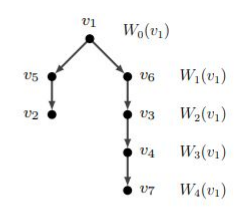
\includegraphics{3_graph}
\end{figure}

$ \left. 
\begin{aligned}
    v_1 &\in W_0 \\ 
    \Gamma _{W_1}(v1) &= \{v_5, v_6\} \\
    \Gamma _{W_2}(v1) &= \{v_2, v_3\} \\
    \Gamma _{W_3}(v1) &= \{v_4\} \\
    \Gamma _{W_4}(v1) &= \{v_7\}
\end{aligned}
\right\} \Rightarrow $ длина кратчайшего пути равна $4$.

\noindent Найдем кратчайший путь:
\begin{enumerate} %[label=\arabic*)]
    \item $v_7$
    \item $ \Gamma_{v_7}^{-1} \cap W_3(v_1) = \{v_4\} \cap \{v_4\} = \{v_4\}$
    \item $ \Gamma_{v_4}^{-1} \cap W_2(v_1) = \{v_3, v_7\} \cap \{v_2, v_3\} = \{v_3\}$
    \item $ \Gamma_{v_3}^{-1} \cap W_1(v_1) = \{v_2, v_4, v_6\} \cap \{v_5, v_6\} = \{v_6\}$
    \item $ \Gamma_{v_6}^{-1} \cap W_0(v_1) = \{v_1, v_2, v_4, v_5\} \cap \{v_1\} = \{v_1\}$
\end{enumerate}
$ v_1 \rightarrow v_6 \rightarrow v_3 \rightarrow v_4 \rightarrow v_7$ - единственный кратчайший путь.
\end{document}